\documentclass[10pt,a4paper]{ctexart}

\usepackage[a4paper,margin=25mm]{geometry}
\usepackage{amsmath}
\usepackage{enumitem}
\usepackage{graphicx}
\usepackage[most]{tcolorbox}
\usepackage{xcolor}
\usepackage{fancyhdr}
\usepackage{titlesec}
\usepackage{microtype}
\usepackage{hyperref}

\graphicspath{{../resources/}}

\definecolor{Terracotta}{HTML}{D97757}
\definecolor{Ink}{HTML}{1F1D1A}
\definecolor{SoftInk}{HTML}{5A554D}
\definecolor{Rule}{HTML}{DDD6C4}
\definecolor{Cream}{HTML}{FAF8F3}
\definecolor{Blue}{HTML}{3B6E8F}
\definecolor{Green}{HTML}{5A8A6A}
\definecolor{Gold}{HTML}{C9A961}

\hypersetup{colorlinks=true,linkcolor=Ink,urlcolor=Blue}
\pagestyle{fancy}
\fancyhf{}
\lhead{第一讲：关于市场}
\rhead{日常制度的经济学}
\cfoot{\thepage}
\renewcommand{\headrulewidth}{0.4pt}

\setlength{\parindent}{2em}
\setlength{\parskip}{0.25em}
\setlist[itemize]{leftmargin=2em,itemsep=0.15em,topsep=0.25em}
\setlist[enumerate]{leftmargin=2.2em,itemsep=0.15em,topsep=0.25em}

\titleformat{\section}{\normalfont\Large\bfseries}{\thesection}{0.8em}{}
\titleformat{\subsection}{\normalfont\normalsize\bfseries}{\thesubsection}{0.8em}{}
\titlespacing*{\section}{0pt}{1.2em}{0.45em}
\titlespacing*{\subsection}{0pt}{0.85em}{0.25em}

\newtcolorbox{goalsbox}{
  enhanced,
  colback=white,
  colframe=Rule,
  boxrule=0.5pt,
  sharp corners,
  left=1.2em,
  right=1.2em,
  top=0.7em,
  bottom=0.8em,
  title=学习目标,
  colbacktitle=SoftInk,
  coltitle=white,
  fonttitle=\bfseries,
  before upper={\setlength{\parskip}{0.45em}}
}

\newtcolorbox{keybox}[1]{
  enhanced,
  breakable,
  colback=Cream,
  colframe=Rule,
  boxrule=0.5pt,
  sharp corners,
  left=1em,
  right=1em,
  top=0.7em,
  bottom=0.7em,
  title=#1,
  colbacktitle=SoftInk,
  coltitle=white,
  fonttitle=\bfseries,
  before upper={\setlength{\parskip}{0.45em}}
}

\newtcolorbox{examplebox}[1]{
  enhanced,
  breakable,
  colback=Cream,
  colframe=Gold,
  boxrule=0.5pt,
  leftrule=2pt,
  sharp corners,
  left=1em,
  right=1em,
  top=0.7em,
  bottom=0.7em,
  title=有趣的例子：#1,
  colbacktitle=Gold,
  coltitle=white,
  fonttitle=\bfseries,
  before upper={\setlength{\parskip}{0.45em}}
}

\newtcolorbox{discussionbox}[1]{
  enhanced,
  breakable,
  colback=Cream,
  colframe=Terracotta,
  boxrule=0.5pt,
  leftrule=2pt,
  sharp corners,
  left=1em,
  right=1em,
  top=0.7em,
  bottom=0.7em,
  before skip=0.8em,
  after skip=0.8em,
  title=讨论：#1,
  colbacktitle=Terracotta,
  coltitle=white,
  fonttitle=\bfseries\small,
  fontupper=\itshape,
  before upper={\setlength{\parskip}{0.45em}}
}

\newtcolorbox{conceptbox}[1]{
  enhanced,
  breakable,
  colback=Cream,
  colframe=Blue,
  boxrule=0.5pt,
  leftrule=2pt,
  sharp corners,
  left=1em,
  right=1em,
  top=0.7em,
  bottom=0.7em,
  title=概念延伸：#1,
  colbacktitle=Blue,
  coltitle=white,
  fonttitle=\bfseries\small,
  before upper={\setlength{\parskip}{0.45em}}
}

\newtcolorbox{insightbox}[1]{
  enhanced,
  breakable,
  colback=Cream,
  colframe=Green,
  boxrule=0.5pt,
  leftrule=2pt,
  sharp corners,
  left=1em,
  right=1em,
  top=0.7em,
  bottom=0.7em,
  title=关键洞察：#1,
  colbacktitle=Green,
  coltitle=white,
  fonttitle=\bfseries,
  before upper={\setlength{\parskip}{0.45em}}
}

\newtcolorbox{questionbox}{
  enhanced,
  breakable,
  colback=Cream,
  colframe=Terracotta,
  boxrule=0.5pt,
  leftrule=1.8pt,
  sharp corners,
  left=1em,
  right=1em,
  top=0.7em,
  bottom=0.7em,
  before skip=0.8em,
  after skip=0.8em,
  title=讨论,
  colbacktitle=Terracotta,
  coltitle=white,
  fonttitle=\bfseries\small,
  fontupper=\itshape,
  before upper={\setlength{\parskip}{0.45em}}
}

\newtcolorbox{notebox}[1]{
  enhanced,
  breakable,
  colback=Cream,
  colframe=Rule,
  boxrule=0.5pt,
  leftrule=1.4pt,
  sharp corners,
  left=1em,
  right=1em,
  top=0.7em,
  bottom=0.7em,
  title=#1,
  colbacktitle=SoftInk,
  coltitle=white,
  fonttitle=\bfseries\small,
  before upper={\setlength{\parskip}{0.45em}}
}

\newcommand{\transitionnote}[1]{%
  \begin{conceptbox}{过渡}#1\end{conceptbox}%
}

\title{\vspace{-2em}\bfseries 第一讲：关于市场}
\author{日常制度的经济学}
\date{Day 1 · What is a market — and where does it end?}

\begin{document}
\maketitle
\thispagestyle{fancy}

\begin{goalsbox}
\begin{itemize}
  \item 对「市场」的概念和基本特征形成初步理解。
  \item 思考市场为什么会出现、为什么有时不会出现，以及市场边界如何受到制度、技术和社会观念的影响。
  \item 初步比较市场机制的优势与局限，为后续讨论福利、外部性、信息不对称和博弈论奠定基础。
\end{itemize}
\end{goalsbox}

\begin{keybox}{课堂主线}
本讲不急于给「市场」下一个标准定义，而是从一组日常与非日常的例子出发，追问两个问题：第一，市场为什么能够在没有统一指挥的情况下协调大量人的需求？第二，如果市场机制如此有效，为什么仍有许多事物不能、也不应完全交给市场来决定？
\end{keybox}

\section{引入：同样是花钱，为什么反应不同？}

\begin{examplebox}{情景对照一：考试}
情景 A：月考前，你花 80 元买了一套《五年高考三年模拟》。这通常不会让人觉得奇怪。

情景 B：月考后，你花 500 元对班里第一名说：「把你的排名让给我。」假设对方也愿意接受。
\end{examplebox}

\begin{examplebox}{情景对照二：时间}
情景 A：晚自习时，你花 15 元叫外卖，骑手用 20 分钟替你跑了一趟。别人的时间被定价了，但多数人不会因此感到不适。

情景 B：18 岁生日时，你花 300 元请一个陌生人陪你过生日。别人的时间同样被定价了，但这一次很多人会觉得不自然。
\end{examplebox}

\begin{discussionbox}{第一反应}
A 和 B 的差别在哪里？是什么让 B 显得不太合适？哪些事物适合用金钱交换，哪些不适合？你的判断依据是什么？
\end{discussionbox}

这些例子说明，市场并不只是「双方自愿、用钱交换」。即使交易双方都同意，我们仍然需要追问：某个事物是否适合被定价？交易会不会改变它原本的意义？它是否会影响第三方，或者破坏某种制度安排？

\begin{conceptbox}{贯穿本讲的两个问题}
市场协调之所以值得研究，是因为它并不依赖一个统一的指挥者，却能够在许多场景中协调大量人的需求。这种协调是如何发生的？

如果市场机制具有如此强的协调能力，为什么仍有许多事物没有交给市场分配？市场的边界在哪里？
\end{conceptbox}

\section{什么是市场？}

可以先从最日常的例子开始。菜市场、股票市场、房地产市场、二手车市场、二手教材市场、辅导班和家教市场，都是比较容易理解的市场。

还有一些例子更容易被忽略：黄牛、代排队服务、考试卷和模拟题的交易。这些现象看起来差异很大，但都有共同点：存在买方和卖方，并且某种价格机制正在发挥作用。

\begin{figure}[h]
\centering

\includegraphics[width=0.72\linewidth]{shijuan.png}
\caption{考试卷和模拟题也可以形成市场。}
\end{figure}

\begin{discussionbox}{市场的最低条件}
如果一次交换中有买方、卖方和价格，这是否已经足以构成一个市场？除此之外还需要哪些条件？
\end{discussionbox}

\section{不太熟悉的市场}

\transitionnote{接下来的例子未必符合我们对「市场」的直觉，但它们确实以市场形式存在。}

\subsection{域名市场：一串字符值多少钱？}

互联网上的每个网站都需要一个域名。域名通常遵循先到先得的注册规则，谁先注册，谁就获得使用权。有人专门低价注册大量域名，等别人需要时再高价转卖。这类似于互联网上的「黄牛」。买家购买的不是一个物理物品，而是互联网上一个独一无二的位置。

一个更戏剧化的例子是 .ai 域名。.ai 原本属于安圭拉（Anguilla），一个加勒比海上人口只有一万多人的英国海外领地。1995 年，这个域名后缀被分配给安圭拉时并没有特殊含义。但 AI 浪潮让它意外变成一项重要资产：claude.ai、perplexity.ai、x.ai、meta.ai、google.ai 都在使用 .ai 域名。2025 年，.ai 域名注册费为安圭拉带来了约 8500 万美元收入，占这个小岛全年国家预算的 47\%。

\subsection{明星祝福视频：注意力也有市场价}

在 Cameo 这样的平台上，用户可以付费请明星或网红录制个性化短视频：生日祝福、求婚助阵，甚至说一句指定的话。不同人的报价差别很大，有人几十美元，有人几千美元。

这里购买的并不只是视频文件本身，而是「这个人专门为我花了 15 秒」所带来的感受。时间、注意力和专属感，都可以被市场定价。

\subsection{Polymarket：给未来定价}

Polymarket 是一个预测市场。对于一个未来事件，例如「2024 年谁会赢得美国大选」，参与者可以用真实资金买入「会」或「不会」。判断正确则获利，判断错误则亏损。所有人的买卖汇总在一起，形成一个价格；这个价格可以被理解为市场对事件发生概率的集体判断。

2024 年美国大选期间，Polymarket 的价格一度被认为比部分民调更敏感地反映了选举预期。

\begin{examplebox}{极端事件也能变成合约}
Polymarket 上曾有一个真实市场：「耶稣会在 2027 年之前重返人间吗？」市场价格隐含的发生概率约为 2\%。这个例子的重点不是宗教判断，而是说明：即使是非常极端、非常抽象的事件，也可以被设计成可交易的合约。

\begin{center}
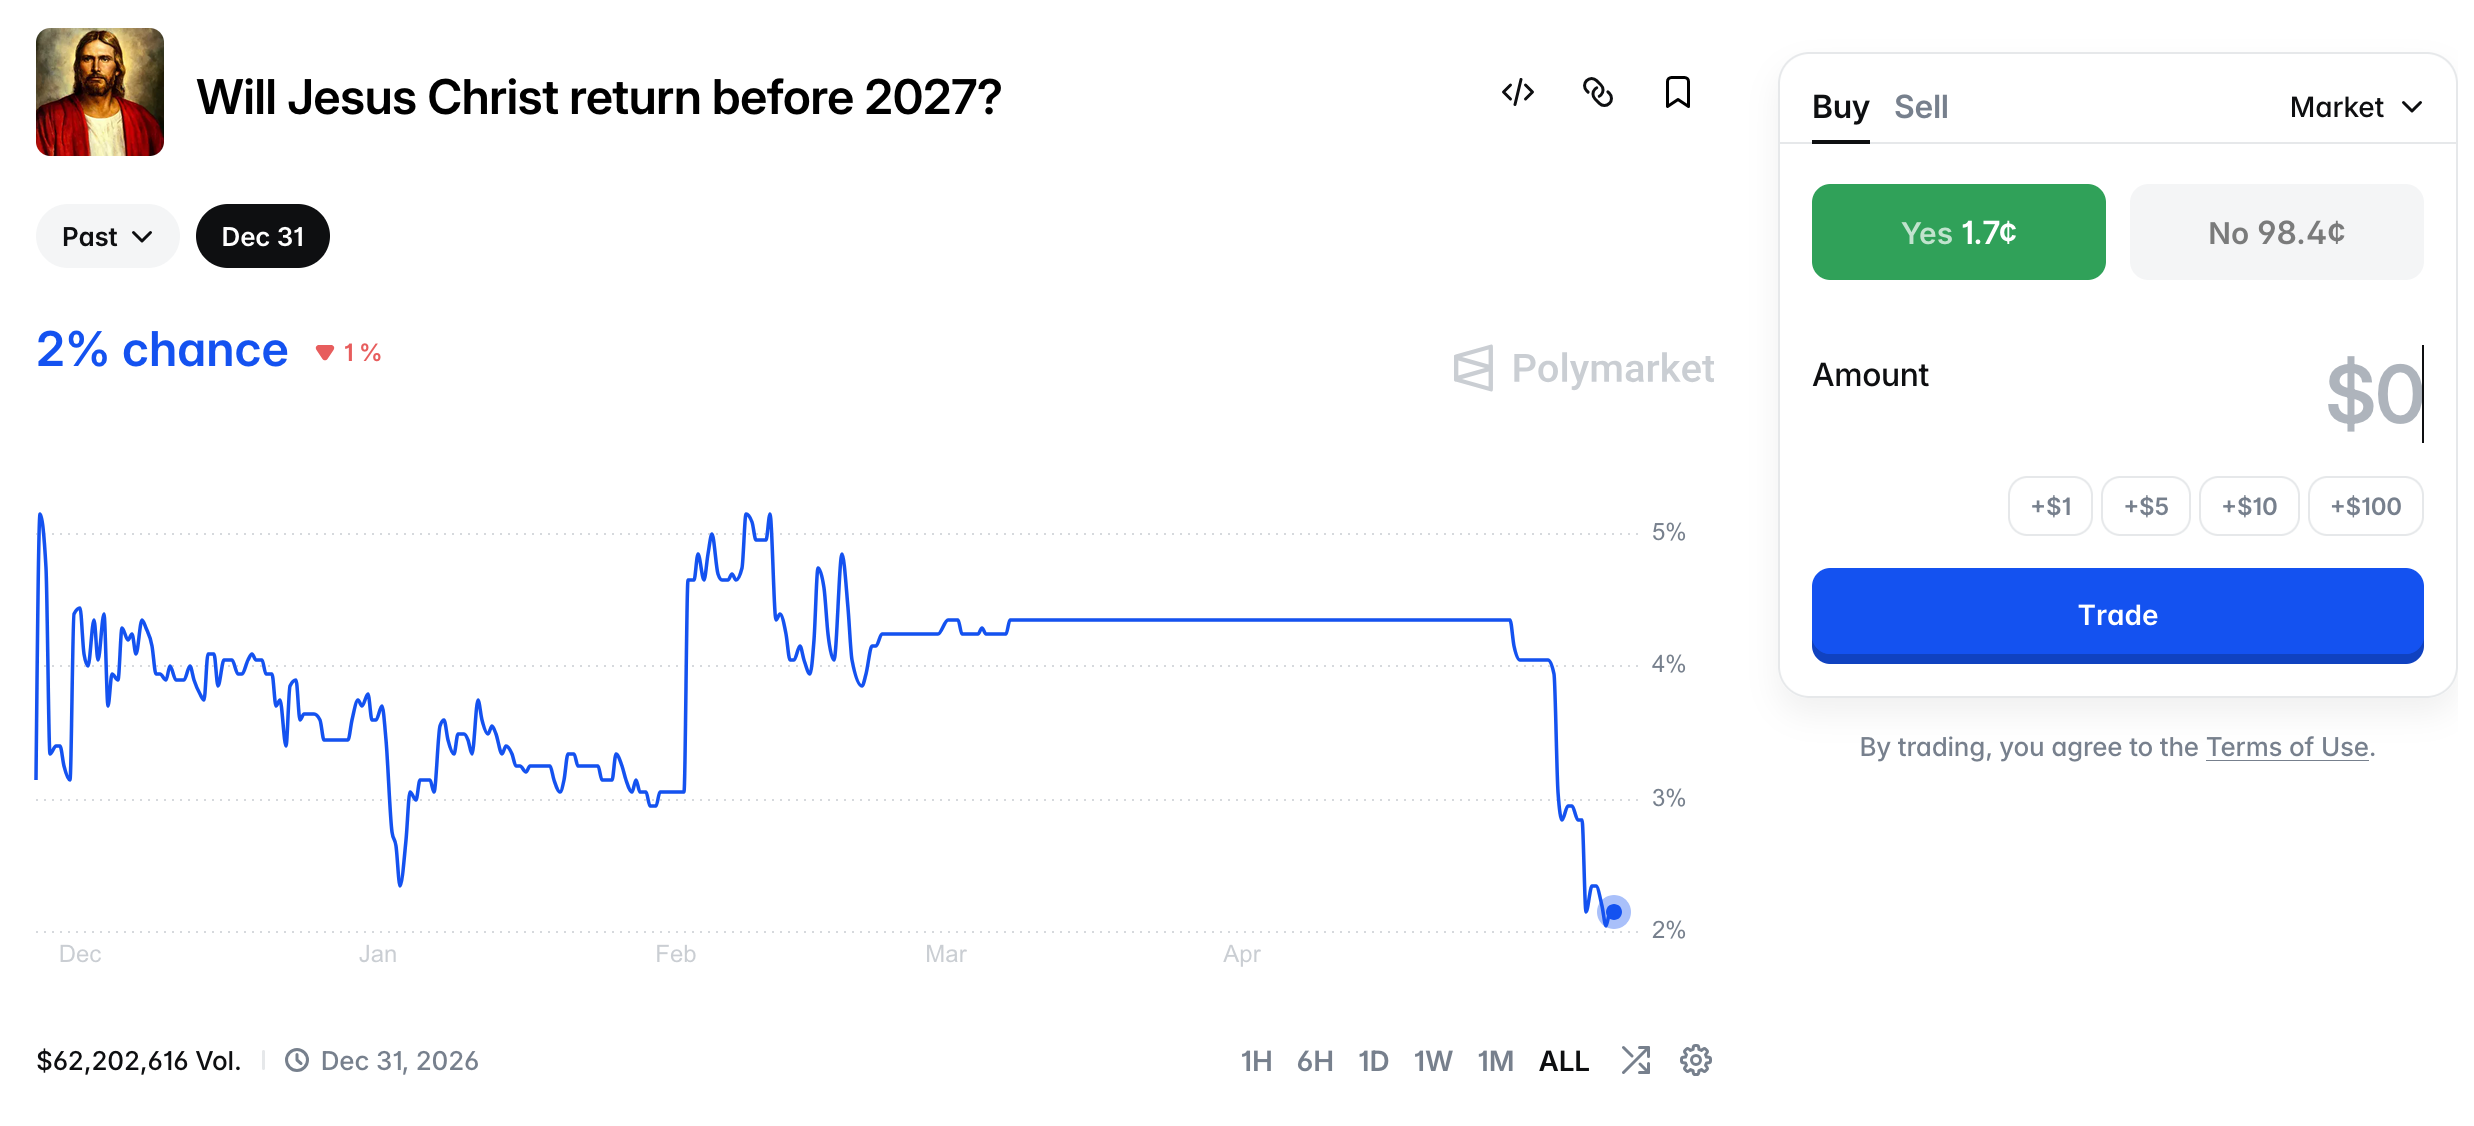
\includegraphics[width=0.76\linewidth]{polymarket.png}
\end{center}
\end{examplebox}

\begin{discussionbox}{预测市场的边界}
为什么会有人创造这种市场？它是在转移风险，还是在制造新的风险？它与赌博的区别在哪里？
\end{discussionbox}

\begin{conceptbox}{保险和预测市场}
保险和 Polymarket 都与未来事件有关：今天支付一笔钱，未来某件事发生或不发生时，这份合约才产生收益。关键区别在于：它是在帮助人们转移和分担风险，还是在创造额外的风险暴露？这类商品不是天然存在的，而是由制度、技术和合约设计共同构造出来的。
\end{conceptbox}

\section{不存在的市场}

\transitionnote{看过「这也能交易」的例子后，可以反过来追问：哪些事物没有市场？}

有些事物表面上似乎可以交易，但现实中通常没有市场；或者即使技术上可以交易，我们也会强烈反对它被交易：考试名次、谁做我的同桌、朋友、求根公式的使用权。

\begin{discussionbox}{不存在的市场}
如果你考了第一名，能把这个名次卖给别人吗？如果双方都愿意呢？你可以花钱请人陪你吃饭，但那能算友谊吗？如果每次使用求根公式都要付费，你能接受吗？
\end{discussionbox}

求根公式是免费的：
\[
x = \frac{-b \pm \sqrt{b^2 - 4ac}}{2a}
\]

但专利可以交易，版权也可以交易。一首歌要收费，一条数学定理通常不收费。两者都属于「知识」，区别在哪里？

关键不在于数学公式的创造不需要激励。恰恰相反，发现一个重要定理、发展一种数学方法、写出一本好教材，都需要长期训练、时间投入和智力劳动。问题在于，这类知识一旦被发现，具有很强的非竞争性：你使用求根公式，并不会减少我使用它的可能性。若每次使用都要收费，社会反而会因为高昂的授权成本而少用知识。

因此，数学和基础科学的激励往往不是通过「每次使用都收取产权费」来实现，而是通过另一套制度来实现：学术声誉、优先发现权、论文发表、职位晋升、奖金、公共资助、学校和研究机构的薪酬，以及学习者和研究者自身的好奇心。这些机制同样是在提供激励，只是它们不一定表现为对每一次使用行为收费。

这说明市场不是唯一的激励机制。产权和价格可以鼓励某些知识产品的生产，例如歌曲、软件、药品和专利技术；但对于基础数学、基础科学和许多公共知识，过强的排他性反而可能阻碍传播和再创造。问题不是「知识要不要激励」，而是「哪一种激励机制更适合这种知识」。

\section{市场在什么条件下可以存在？}

\begin{discussionbox}{市场存在的条件}
市场「可以存在」是否意味着它一定会出现？如果不是，还需要哪些条件？
\end{discussionbox}

\begin{enumerate}
  \item \textbf{商品：稀缺性与可交易性。} 没有稀缺性，就没有定价的必要。空气在很多时候不是商品，但雾霾会让洁净空气的价值间接体现在房价和人口流动中。物品的性质也必须允许交易：求根公式「你用了不影响我用」，这类知识很难排除他人使用并收费。
  \item \textbf{交易的动机。} 如果每个人自己完成一件事和通过交易完成一样有效，就没有交易的必要。市场存在的前提是交易能够让参与者获得收益。
  \item \textbf{参与者。} 市场需要足够多的买家和卖家，或者商品本身的价值得到一定程度的承认。互联网大幅降低了寻找交易对象的成本。
  \item \textbf{价格形成机制。} 价格如何形成？通过拍卖、协商，还是竞争？供给与需求如何塑造价格，是市场运行的核心问题。
  \item \textbf{制度基础设施。} 产权制度、信息披露、评价系统、准入门槛和法律执行，都有助于降低交易成本和信任成本。没有这些制度，市场也可能存在，但交易规模会明显受限。
  \item \textbf{技术条件。} 搜索、匹配、执行和监管技术可以让原本难以形成的市场变得可行。淘宝和京东降低了搜索成本；区块链技术让 Polymarket 的交易更难被篡改；碳排放权交易需要排放监测技术。
\end{enumerate}

\begin{insightbox}{市场不是自然物}
市场并不是自然而然出现的。很多时候，连「什么可以成为商品」这一点本身，也需要由制度、技术和社会观念共同塑造。
\end{insightbox}

\begin{conceptbox}{市场边界由谁画出？}
肾脏交易在伊朗合法，在中国不合法。碳排放权交易则需要政府先界定「排放权」这一交易对象，市场才可能形成。为什么大多数人觉得买卖友谊不可接受？为什么大学录取名额不能拍卖？这些边界是谁划定的？道德和文化条件也是市场能否存在的一部分，只是常常被忽视。
\end{conceptbox}

\section{如果不用市场，还能怎么分配？}

市场不是唯一的分配方式。稀缺资源可以通过很多机制决定由谁获得。

\begin{itemize}
  \item \textbf{排队（先到先得）：} 春运火车票、医院挂号、食堂打饭。成本不是钱而是时间，对时间充裕的人有利。
  \item \textbf{抽签（随机分配）：} 车牌摇号、某些学校的入学名额。它看似公平，但通常不考虑谁更需要。
  \item \textbf{行政分配（按标准）：} 医院急诊按病情严重程度排序，保障房按收入水平分配。需要有人制定标准，而标准本身可以被博弈。
  \item \textbf{按权力或关系：} 「找人帮忙」「走后门」。非正式，但普遍存在。
  \item \textbf{考试或竞争：} 高考分配大学名额。它以能力或至少以考试成绩作为分配依据，但考试结果本身也可能受到补习、家庭资源和学区房等因素影响。
\end{itemize}

每种方式都有各自的效率与公平问题，没有一种机制是完美的。

\begin{insightbox}{市场会从缝隙里长出来}
选择不用市场分配，并不意味着市场力量会消失。火车票采用排队分配，黄牛可能出现，用金钱替代时间；医院挂号采用行政分配，号贩子可能出现；车牌采用摇号分配，租牌市场可能出现。只要稀缺性存在，新的交易形式就可能在制度缝隙中自发生成。
\end{insightbox}

\section{市场带来了什么？}

市场能够存在，并不意味着它一定带来好的结果。评价一个市场时，不应只问「市场好不好」，而应追问：它在具体情境中解决了什么问题，又带来了什么新的问题？

\begin{discussionbox}{市场的利弊}
市场存在与不存在，各有什么利弊？请结合实际例子，说明市场机制可能带来的正面或负面影响。
\end{discussionbox}

\subsection{六个讨论案例}

\begin{itemize}
  \item \textbf{口罩的二级市场：} 疫情期间，口罩价格一度大幅上涨。这个市场是让口罩流向更愿意付费的人，还是让支付能力较弱的人更难获得口罩？
  \item \textbf{学区房：} 学位无法直接买卖，但通过房产市场，优质教育资源事实上被定价了。这让教育不平等更加可见，还是进一步加剧了不平等？
  \item \textbf{演唱会黄牛：} 官方售价几百元的票被转卖到几千元。有人认为这是价格机制的体现，有人认为这是对普通消费者的挤出。
  \item \textbf{医疗市场化：} 当医疗服务高度依赖市场交易，而患者又很难判断质量时，会发生什么？莆田系医院的问题可以作为一个讨论案例。
  \item \textbf{外卖平台：} 平台让小餐馆触达更多顾客，但也可能把骑手置于算法制造的时间压力之下。市场扩大了，但谁受益，谁承担成本？
  \item \textbf{名校参观黄牛：} 北大清华暑假参观名额很快被抢空，黄牛以数百元价格转卖预约名额。免费的公共资源因为需求过大变成了稀缺品，市场交易随之出现。
\end{itemize}

\subsection{怎么评价一个市场？}

\begin{enumerate}
  \item \textbf{效率：} 资源是否被更有效地使用？价格能否帮助人们发现谁更需要、哪里更短缺、什么更值得生产？
  \item \textbf{分配：} 谁获得了资源，谁被排除在外？市场通常按照支付能力分配，但支付能力不一定等于真实需要。
  \item \textbf{边界：} 交易是否会改变事物的意义？有些事物一旦被定价，关系、信任或公共价值本身就可能发生变化。
\end{enumerate}

\subsection{市场的力量}

市场是一种常常有效、但并不万能的协调机制。它之所以顽强，至少有几个原因：价格携带着分散在无数人头脑中的信息；利润和亏损提供激励，使资源更容易流向短缺之处；专业化和分工提高效率；竞争迫使卖家不断回应买家的需求，否则就可能被替代。

Adam Smith 的经典洞察是：我们的晚餐不是来自屠夫、酿酒师和面包师的慈悲，而是来自他们对自己利益的关注。

\subsection{市场的代价}

\begin{itemize}
  \item \textbf{支付能力不等于真实需要。} 学区房、口罩、演唱会门票都可能把资源分给出价最高的人，而不是最需要的人。
  \item \textbf{信息不对称。} 在医疗、二手车、教育服务中，买方往往很难判断质量，价格也未必代表真实价值。
  \item \textbf{外部成本。} 外卖更方便，但时间压力可能被转嫁给骑手；交易双方之外的人也可能承担后果。
  \item \textbf{意义被改变。} 友谊、荣誉、公共资源一旦被买卖，原本的社会意义可能被价格重新定义。
\end{itemize}

\section{市场的边界与后续问题}

\begin{discussionbox}{边界问题}
市场的边界在哪里？这是道德边界，还是功能边界？如果某种事物可以被买卖，是否意味着它就应该被买卖？
\end{discussionbox}

有些事物并非不能被定价，而是我们不愿意让它被定价。另一些事物并非我们不愿意定价，而是一旦定价，原本的意义或功能就可能被破坏。

\subsection{两种边界}

\begin{itemize}
  \item \textbf{功能边界：} 有些事物市场很难处理，例如难以排他的知识、难以观察质量的医疗服务、交易前后信息严重不对称的商品，以及影响会扩散到交易双方之外的活动。在这些场景中，市场机制的问题不一定在于「不道德」，而在于它未必能稳定地产生好结果。
  \item \textbf{道德边界：} 有些事物即使可以交易，我们也会认为不应该交易，例如友谊、尊严、投票权、学位、某些公共荣誉。Michael Sandel 提出的问题可以作为引入：如果一切都可以买卖，社会关系会发生什么变化？
\end{itemize}

\subsection{怎么判断总体好坏？}

市场带来的好处和坏处，往往不只是金钱本身，还包括时间、风险、尊严、机会、公平感和幸福感。

\begin{discussionbox}{衡量标准}
如果这些价值不能简单相加，我们凭什么说一种制度「总体更好」？是否必须先选择某种衡量标准？
\end{discussionbox}

这会引向下一讲「快乐的度量学」。我们会讨论效用、福利，以及衡量标准本身的问题。

\subsection{复杂互动如何研究？}

经济学并不是把现实简单化到失真，而是先把复杂互动整理成一个可以分析的结构：

\begin{itemize}
  \item \textbf{Players：} 谁在互动？消费者、商家、平台、政府、旁观者。
  \item \textbf{Actions：} 他们可以做什么？购买、拒绝购买、涨价、排队、绕开规则。
  \item \textbf{Payoffs：} 他们在乎什么？金钱、时间、风险、声誉、公平感。
  \item \textbf{Rules / Game structure：} 规则是什么？价格、法律、平台算法、学校制度。
  \item \textbf{Information：} 谁知道什么？质量、成本、风险、真实意图。
  \item \textbf{Outcome：} 结果如何产生？它未必由某个人单独设计出来，而是在互动中形成的。
\end{itemize}

模型不是现实本身，而是帮助我们更有纪律地思考现实。

\section{后面几讲的问题地图}

这门课后面会反复追问：

\begin{itemize}
  \item 如果快乐、风险和公平很难被直接统计，我们如何比较不同制度的好坏？
  \item 如果一个人的交易会影响第三方，市场价格还能完整反映真实成本吗？
  \item 如果买卖双方掌握的信息不同，市场还会稳定地产生好结果吗？
  \item 如果社会结果来自许多人的互动，我们需要怎样的模型来理解它？
\end{itemize}

\end{document}
